 \documentclass[c]{beamer}
%\documentclass{beamer}
\listfiles

\mode<presentation>
{
  %\usetheme[deutsch,titlepage0]{KIT}
\usetheme[deutsch]{KIT}
% \usetheme{KIT}

%%  \usefonttheme{structurebold}

  \setbeamercovered{transparent}

  \setbeamertemplate{enumerate items}[circle]
  %\setbeamertemplate{enumerate items}[ball]

}
\usepackage{babel}
\date{}
%\DateText

\newlength{\Ku}
\setlength{\Ku}{1.43375pt}

\usepackage[utf8]{inputenc}
\usepackage[TS1,T1]{fontenc}
\usepackage{array}
\usepackage{multicol}
\usepackage{lipsum}
\usepackage[]{algorithm2e}
\usepackage{amsmath}
\usepackage{color}

\usenavigationsymbols
%\usenavigationsymbols[sfHhdb]
%\usenavigationsymbols[sfhHb]

\subtitle{Algorithmen I SS 14}
\author[]{Vincent Schüßler}

\AuthorTitleSep{\relax}

\institute[ITI]{Institut für Theoretische Informatik}

\TitleImage[width=\titleimagewd]{images/title}

\newlength{\tmplen}

\newcommand{\verysmall}{\fontsize{6pt}{8.6pt}\selectfont}

\title[Algorithmen I SS 14]{Tutorium 8}

\usepackage{alltt}

\TitleImage[width=\titleimagewd]{images/title02}

\begin{document}

\begin{frame}
  \maketitle
\end{frame}

\begin{frame}
	\begin{center}
		\Huge
		Graphtraversierung
	\end{center}
\end{frame}

\begin{frame}{Breitensuche (BFS)}
	\begin{itemize}
		\item Funktionsweise:
			\begin{enumerate}
				\item Beginne bei einem Startknoten $s$
				\item Besuche alle (unbesuchten) Nachbarknoten von $s$
				\item Besuche die Nachbarknoten dieser Knoten
				\item …
			\end{enumerate}
		\item Implementierung über Queue
		\item Graph wird "`Schichtenweise"' durchgegangen (Abstand zum Startknoten)
	\end{itemize}
\end{frame}

\begin{frame}{Bipartite Zerlegung}
	\begin{itemize}
		\item Ein Graph $G = (V, E)$ heißt bipartit $:\Leftrightarrow \exists A, B \subseteq V: A \cap B = \varnothing, A \cup B = V  \wedge  \forall (u, v) \in E: (u, v) \in ((A \times B) \cup (B \times A))$
		\item Also: die Knoten lassen sich in zwei Mengen aufteilen, so dass es keine Kanten innerhalb der Knoten in einer Menge gibt
		\item Aufgabe: Entwickle einen Algorithmus, der für einen ungerichteten, zusammenhängenden Graphen eine bipartite Zerlegung findet (oder erkennt, dass keine existiert). Laufzeit: $\mathcal{O}(|E|)$
	\end{itemize}
\end{frame}

\begin{frame}{Tiefensuche (DFS)}
	\begin{itemize}
		\item Funktionsweise:
			\begin{enumerate}
				\item Beginne bei einem Startknoten $s$
				\item Besuche den ersten (unbesuchten) Nachbarknoten von $s$
				\item Besuchen den ersten Nachbarknoten dieses Knotens
				\item …
				\item Besuche den zweiten Nachbarknoten von $s$
				\item …
			\end{enumerate}
		\item Intuitiv rekursiv
		\item Iterative Implementierung?
	\end{itemize}
\end{frame}

\begin{frame}{Kantenklassifizierung}
	\begin{center}
		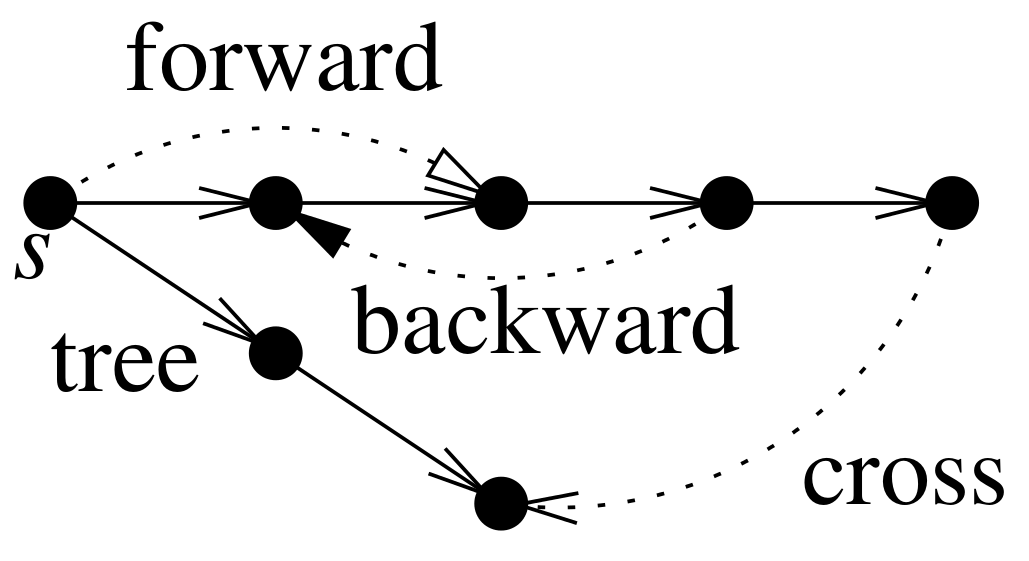
\includegraphics[keepaspectratio,scale=0.25]{images/edges}
	\end{center}
\end{frame}

\begin{frame}{Topologische Sortierung}
	\begin{itemize}
		\item Sortiere die Knoten eines Graphen nach der Relation $a \leq b :\Leftrightarrow \text{Es gibt einen Pfad von a nach b}$
		\item Lösung über modifizierte Tiefensuche:
			\begin{enumerate}
				\item Speichere "`Zeitpunkt"' des Knotenabschlusses (keine Nachbarn mehr)
				\item Falls Rückwärtskante gefunden wird $\Rightarrow$ Abbruch
				\item Sortiere die Knoten absteigend nach Abschlusszeit
			\end{enumerate}
		\item Aufgabe: Wie kann Breitensuche modifiziert werden, um eine topologische Sortierung zu berechnen?
	\end{itemize}
\end{frame}

\begin{frame}
	\begin{center}
		\Huge
		Wiederholung
	\end{center}
\end{frame}

\begin{frame}{Themen}
	\begin{itemize}
		\item O-Kalkül, Mastertheorem
		\item Invarianten, Korrektheit von Algorithmen
		\item Verkettete Listen (einfach und doppelt)
		\item Unbounded Arrays
		\item Stack, Queue, Deque
		\item Hashing, Hashtabellen
		\item Sortieren
			\begin{itemize}
				\item Insertionsort
				\item Mergesort
				\item Quicksort (Quickselect)
				\item Heapsort
				\item Bucketsort
				\item Radixsort
			\end{itemize}
		\item Heaps
		\item (Binäre) Suchbäume
		\item Graphen
	\end{itemize}
\end{frame}

\begin{frame}{Aufgaben}
	Zeigen oder widerlegen Sie, dass $2^{3n} = \mathcal{O}(5^n)$
\end{frame}

\begin{frame}{Aufgaben}
	Bestimmen Sie die Lösung der folgenden Rekurrenz im $\Theta$-Kalkül mit dem Master-Theorem:
	$$ T(1) = 5, T(n) = n + 2 S(n/2), n = 2^k, k \in \mathbb{N}$$
\end{frame}

\begin{frame}{Aufgaben}
	Nennen Sie zwei Operationen, die doppelt verkettete Listen in konstanter worst-case-Zeit unterstützen, einfach verkettete Listen jedoch nicht.
\end{frame}

\begin{frame}{Aufgaben}
	Nennen Sie einen Vorteil und einen Nachteil von einfach verketteten Listen gegenüber unbeschränkten Feldern.
\end{frame}

\begin{frame}{Aufgaben}
	Wie lautet die Invariante für doppelt verkettete Listen aus der Vorlesung?
\end{frame}

\begin{frame}{Aufgaben}
	Nennen Sie einen Vorteil und einen Nachteil von Hashing mit verketteten Listen gegenüber offenem Hashing mit linearer Suche.
\end{frame}

\begin{frame}{Aufgaben}
	Nennen sie einen Vorteil und einen Nachteil von Mergesort gegenüber Quicksort.
\end{frame}

\begin{frame}{Aufgaben}
	Wie lautet die Heap-Eigenschaft?
\end{frame}

\begin{frame}{Aufgaben}
	Nennen Sie einen Vorteil und einen Nachteil von Adjazenzfeldern gegenüber Adjazenzlisten.
\end{frame}

\begin{frame}{Kreativaufgabe}
	Gegeben sei ein stark zusammenhänger Graph in folgender Darstellung:

	\begin{itemize}
		\item Knotenarray: Für jeden Knoten ID und Zeiger auf Array mit Kanten
		\item Kantenarray: Für jede Kante ID der Kante und ID des Zielknotens
	\end{itemize}

	Entwirf eine abgewandelte BFS, die \emph{in-place} arbeitet, also nur $\mathcal{O}(1)$ zusätzlichen Platz benötigt.
	Die Laufzeit darf schlechter sein als eine herkömmliche Breitensuche.
\end{frame}

\begin{frame}{DFS}
	\begin{center}
		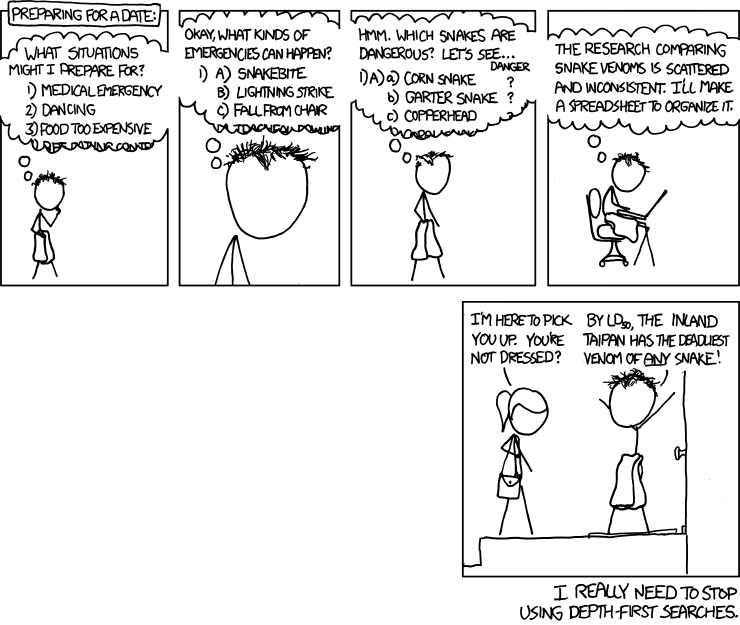
\includegraphics[width=\textwidth,height=\textheight,keepaspectratio]{images/dfs}
	\end{center}
\end{frame}

\end{document}
